%!TEX TS-program = xelatex
\documentclass[aspectratio=169]{beamer}

%\usepackage{HSE-theme/beamerthemeHSE} % Load HSE theme

\usetheme{default}

%%% Fonts 
\usepackage{fontspec}
\defaultfontfeatures{Ligatures={TeX},Renderer=Basic}
\setmainfont[Ligatures={TeX,Historic}]{Myriad Pro} % install Myriad Pro or replace with Arial
\setsansfont{Myriad Pro}  % install Myriad Pro or replace with Arial
\setmonofont{Courier New}
\uselanguage{russian}
\languagepath{russian}
\deftranslation[to=russian]{Theorem}{Теорема}
\deftranslation[to=russian]{Definition}{Определение}
\deftranslation[to=russian]{Definitions}{Определения}
\deftranslation[to=russian]{Corollary}{Следствие}
\deftranslation[to=russian]{Fact}{Факт}
\deftranslation[to=russian]{Example}{Пример}

\usepackage{multicol} 		% Multiple columns
\setlength{\multicolsep}{6.0pt plus 2.0pt minus 1.5pt}
\usepackage{graphicx}
\graphicspath{{images/}}  	% Images folder

\usepackage{tabularx}
\usepackage{cases}

%\setbeamertemplate{frametitle} % Frametitle with logo
%{
%	\nointerlineskip
%	\begin{beamercolorbox}[sep=0.3cm,wd=\paperwidth]{frametitle}
%		\vbox{}\vskip-0.7ex% 
%		\begin{wrapfigure}{r}{0.10\textwidth}
%			\vskip-3ex\includegraphics[width=0.06\textwidth]{HSE-theme/HSE-small}
%		\end{wrapfigure}
%		\strut\insertframetitle \strut\ ---\ \insertframesubtitle
%		\vskip-0.8ex%
%	\end{beamercolorbox}
%}

\setbeamertemplate{navigation symbols}{}

\setbeamertemplate{footline}{% 
	\hfill% 
	\usebeamercolor[fg]{page number in head/foot}% 
	\usebeamerfont{page number in head/foot}% 
	\insertframenumber%
	%\,/\,\inserttotalframenumber
	\kern1em\vskip2pt% 
}
%\setbeamerfont{page number in head/foot}{size=\tiny}
%\setbeamertemplate{footline}[frame number]

%%% Author and speech
\title{Метод обобщения в таксономиях и его применение} 
\subtitle{Method for Appropriate Generalization in a Taxonomy}
\author[Власов А.С.]{\texorpdfstring{%
		\vspace{0.7cm}
		\footnotesize
		\begin{minipage}{.5\textwidth}
			\begin{flushleft}
				Выполнил: \\
			Власов Александр Сергеевич \\
			студент группы мНоД17-ИССА
			\end{flushleft}
		\end{minipage}%  
		\begin{minipage}{.5\textwidth}
			\begin{flushright}
			Руководитель: \\
			Миркин Борис Григорьевич \\
			д.т.н. профессор
			\end{flushright}
	\end{minipage}}{}}

\institute[ФКН НИУ ВШЭ]{
	Национальный исследовательский университет \\ «Высшая школа экономики» \vspace{5pt} \\  Факультет компьютерных наук \vspace{-7pt}
} 

\date[2019]{
	\texorpdfstring{
		\tiny
		13 июня 2019
	}{}
}


\begin{document}	% Document begins


\frame[plain]{\titlepage}	% Title frame
\begin{frame}
\frametitle{Содержание}
\tableofcontents
\end{frame}

%%%%%%%%%%%%%%%%%%%%%%%%%%%%%%%%%%%%%%%%
\section{Цели работы}

\begin{frame}
\frametitle{\insertsection}
\framesubtitle{\insertsubsection}
\begin{itemize}
	\item Применить метод оптимального обобщения, разработанный Фроловым Д.С. и Миркиным Б.Г. \footnote{Finding an appropriate generalization for a fuzzy thematic set in taxonomy / Dmitry Frolov [и др.] // Series WP7 "Математические методы анализа решений в экономике, бизнесе и политике". — 2018. — Т.4.}, к анализу тенденций развития науки о данных.
	\item Предложить модификацию метода для критерия максимального правдоподобия.
	\item Провести экспериментальное исследование на расширенной текстовой коллекции.
\end{itemize}
\end{frame}

\section{Таксономия и обобщение в таксономии}

\begin{frame}
	\frametitle{\insertsection}
	\framesubtitle{Фрагмент таксономии компьютерных наук ACM Computing Classification System 2012}
	\begin{figure}
		\centering
		\includegraphics[width=0.9\linewidth, clip]{images/ds_tax_fragment}
	\end{figure}
\end{frame}

\begin{frame}
	\frametitle{\insertsection}
	\framesubtitle{Тривиальный пример}
	\begin{figure}
	\centering
	%	\hspace{-1.4cm}
	\includegraphics[width=0.9\linewidth, clip]{images/lift_ex_trivial}
	\end{figure}
\end{frame}

\begin{frame}
	\frametitle{\insertsection}
	\framesubtitle{Тривиальный пример: обобщение}
	\begin{figure}
		\centering
		%	\hspace{-1.4cm}
		\includegraphics[width=0.9\linewidth, clip]{images/lift_ex_trivial_g}
	\end{figure}
\end{frame}

\begin{frame}
	\frametitle{\insertsection}
	\framesubtitle{Нетривиальный пример}
	\begin{figure}
		\centering
		%	\hspace{-1.4cm}
		\includegraphics[width=0.9\linewidth, clip]{images/lift_ex_nontriv}
	\end{figure}
\end{frame}

\begin{frame}
\frametitle{\insertsection}
\framesubtitle{Нетривиальный пример: обобщение 1}
\begin{figure}
	\centering
	%	\hspace{-1.4cm}
	\includegraphics[width=0.9\linewidth, clip]{images/lift_ex_nontriv_g1}
\end{figure}
\end{frame}
\begin{frame}
\frametitle{\insertsection}
\framesubtitle{Нетривиальный пример: обобщение 2}
\begin{figure}
\centering
%	\hspace{-1.4cm}
\includegraphics[width=0.9\linewidth, clip]{images/lift_ex_nontriv_g2}
\end{figure}
\end{frame}


\subsection{Метод наибольшей экономии}
\begin{frame}
	\frametitle{Выбор оптимального обобщения}
	\framesubtitle{\insertsubsection}
	Идея: оптимальное обобщение имеет \emph{наименьшее} количество элементов (головных понятий, пробелов, выбросов).
	
	Штрафная функция:
	\begin{equation*}
	p(H)=\sum_{h\in \textsf{heads}(H)}u(h) + \sum_{h\in \textsf{heads}(H)}\sum_{g\in G(h)}\lambda v(g) + \sum_{h\in \textsf{offshoots}(H)}\gamma u(h)
	\label{eq:pars_criterion}
	\end{equation*}
	\begin{itemize}
		\item $u(\cdot)$ --- функция принадлежности, определенная на листьях таксономии,
		\item 1 --- штраф за головное понятие
		\item $\gamma$ --- штраф за пробел,
		\item $\lambda$ --- штраф за выброс.
	\end{itemize}
\end{frame}

\subsection{Метод максимального правдоподобия}

\begin{frame}
	\frametitle{Выбор оптимального обобщения}
	\framesubtitle{Метод максимального правдоподобия (собственная разработка)}
	Идея: максимизировать вероятность \textbf{сценария}.
	\begin{itemize}
		\item Каждой вершине в соответствие ставится событие: приобретение, потеря или передача головного понятия.
		\item Сценарий: множество событий в каждой из вершин.
	\end{itemize}
	~\\
	
	Особенности:
	\begin{itemize}
		\item Не требует явного задания штрафных коэффициентов.
		\item Использует априорные вероятности приобретений и потерь головных понятий в вершинах.
	\end{itemize}	
\end{frame}

\newcommand{\ScIt}{Sc_t^I}
\newcommand{\ScNt}{Sc_t^N}
\newcommand{\ScIw}{Sc_w^I}
\newcommand{\ScNw}{Sc_w^N}
\newcommand{\children}[1] {\textsf{C}(#1)}
\newcommand{\pInhLost}{p_t^\text{loss}\prod_{w\in\children{t}}p(\ScNw)}
\newcommand{\pInhPass}{(1-p_t^\text{loss})\prod_{w\in\children{t}}p(\ScIw)}
\newcommand{\pNotInhGain}{p_t^\text{gain}\prod_{w\in\children{t}}p(\ScIw)}
\newcommand{\pNotInhPass}{(1-p_t^\text{gain})\prod_{w\in\children{t}}p(\ScNw)}

\begin{frame}
	\frametitle{Выбор оптимального обобщения}
	\framesubtitle{Наследование}
	\begin{columns}
		\column{.5\linewidth}
		I. Головное понятие \emph{унаследовано} от родителя:
		\begin{figure}
			\centering
			%	\hspace{-1.4cm}
			\includegraphics[width=0.9\linewidth, clip]{images/mals_inher}
		\end{figure}
		\begin{equation*}
		p(\ScIt) = \max\begin{cases}
		\pInhLost,\\
		\pInhPass;
		\end{cases}
		\end{equation*}
		
		\column{.5\linewidth}
		II. Головное понятие \emph{не унаследовано} от родителя:
		\begin{figure}
			\centering
			%	\hspace{-1.4cm}
			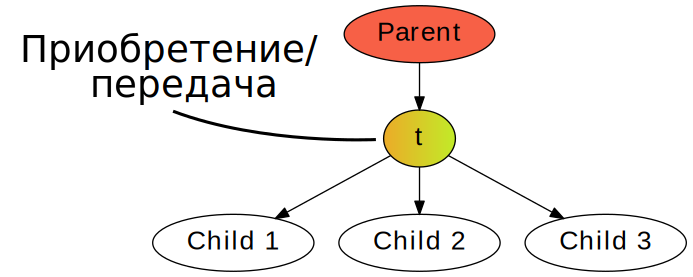
\includegraphics[width=0.9\linewidth, clip]{images/mals_notinher}
		\end{figure}
		\begin{equation*}
		p(\ScNt) = \max\begin{cases}
		\pNotInhGain, \\
		\pNotInhPass;
		\end{cases}
		\end{equation*}
		
	\end{columns}
	
	
	
	
\end{frame}


\begin{frame}
\frametitle{Выбор оптимального обобщения}
\framesubtitle{Пример сценария}
\begin{figure}
	\centering
	%	\hspace{-1.4cm}
	\includegraphics[width=0.9\linewidth, clip]{images/scenario_example}
\end{figure}
\end{frame}

\section{Схема применения метода обобщения}

\subsection{Коллекция текстов и таксономия науки о данных}

\begin{frame}
	\frametitle{\insertsection}
	\framesubtitle{\insertsubsection}
	\begin{itemize}
		\item 26 799 аннотаций статей в области Data Science из 80 журналов издательств Springer и Elsevier за период 1971 - 2018 гг.
		
		
		\begin{table}
%			\def\arraystretch{0.9}
			\centering
			{\footnotesize
				\begin{tabular}{|l|r|r|l|}
					\hline
					Название журнала                                    &  \# Cтатей     & \# Томов & Период     \\
					\hline
					Neurocomputing                                      &  3187 &  334 &  1992--2019 \\
					Expert Systems with Applications                    &  2033 &  243 &  1998--2019 \\
					Procedia Computer Science                           &  1933 &  139 &  2010--2019 \\
					Pattern Recognition                                 &  1360 &  301 &  1973--2019 \\
					Applied Soft Computing                              &  1236 &  117 &  2003--2019 \\
					Information Sciences                                &  1211 &  350 &  1998--2019 \\
					Pattern Recognition Letters                         &  1001 &  292 &  1982--2019 \\
					\hline
			\end{tabular}}
		\end{table}
	
		\item Таксономия Data Science, основанная на ACM Computing Classification System:
		\begin{itemize}
			\item максимальная глубина равна 7,
			\item 456 вершин,
			\item 353 листа.
		\end{itemize}
	
		
	\end{itemize}
	
%	\begin{figure}
%		\centering
%		\includegraphics[width=0.5\linewidth, clip]{images/ds_tax_fragment_2upper}
%	\end{figure}

\end{frame}

\subsection{Тематические кластеры на листьях таксономии}
	
	
\begin{frame}
	\frametitle{\insertsection,~1}
	\framesubtitle{\large \insertsubsection}
	Этапы расчетов:
	\begin{enumerate}
		\item Построение матрицы релевантности $\mathcal{R}$ текстов к листьям таксономии с помощью метода \textbf{аннотированного суффиксного дерева} ($26799\times353$). 
		\item Расчет матрицы $\mathcal{C}$ корелевантности листьев таксономии как взвешенного матричного произведения $\mathcal{R}^T$ и $\mathcal{R}$ ($353\times353$) . 
		\item Применение \textbf{псевдо-обратного преобразования Лапласа} (LAPIN).
		\item Извлечение тематических кластеров на листьях таксономии с помощью метода \textbf{нечеткой аддитивной спектральной кластеризации} (FADDIS).
	\end{enumerate}
\end{frame}


\subsection{Оптимальное обобщение}


\begin{frame}
\frametitle{\insertsection,~2}
\framesubtitle{\large \insertsubsection}

Полученные тематические кластеры обобщаются двумя методами:
\begin{enumerate}
	\item Методом наибольшей экономии (алгоритм \textbf{ParGenFS}),
	\item Методом максимального правдоподобия (алгоритм \textbf{MalGenFS}).
\end{enumerate}
~\\

Далее:
\begin{enumerate}
	\item Обобщенные кластеры интерпретируются,
	\item Проводится сравнение с ранними результатами,
	\item Методы обобщения (исходный и модифицированный) сравниваются между собой.
\end{enumerate}


\end{frame}



\section{Результаты экспериментов}

\begin{frame}
\frametitle{\insertsection}
\framesubtitle{Тематические кластеры}
\begin{itemize}
	\item  На 26 799 аннотациях статей получено 35 тематических кластеров, к ним применены методы обобщения.
	\item  7 обобщенных кластеров оказались хорошо интерпретируемыми:
	\begin{multicols}{2}
		\begin{itemize}
			\item Learning
			\item Clustering
			\item Probabilistic representations
			\item Structuring
			\item Computer vision representations
			\item Retrieval и Querying
		\end{itemize}
	\end{multicols}
	\item Похоже на более ранние результаты Фролова и Миркина на 17000 статей:
	\begin{itemize}
		\item \textbf{Learning}: в точности совпадает с полученным в данной работе.
		\item \textbf{Clustering}: более плотный и содержит меньше головных понятий и выбросов.
		\item \textbf{Retrieval}: разделен на несколько более маленьких кластеров.
	\end{itemize}
\end{itemize}

\end{frame}

\begin{frame}
	\frametitle{\insertsection}
	\framesubtitle{Визуализация кластера Learning на таксономии}
	\begin{figure}
	%	\centering/
		\includegraphics[width=1.\linewidth, clip]{images/cluster_lift_tree_00_learning}
	\end{figure}

\end{frame}

\begin{frame}
	\frametitle{\insertsection}
	\framesubtitle{Сравнение методов оптимального обобщения}
	
	\begin{enumerate}
		\item Исходный алгоритм: метод наибольшей экономии,
		\item Модифицированный алгоритм: метод максимального правдоподобия.
	\end{enumerate}
	Результат работы модифицированного алгоритма \textbf{практически полностью совпал} с исходным алгоритмом.\\
	~\\
	
	При этом модифицированный алгоритм:
	\begin{itemize}
		\item Работает только с \emph{жесткими} кластерами.
		\item Не требует явного задания параметров штрафа за выбросы и пробелы. 
	\end{itemize}

\end{frame}

\section{Заключение}

\begin{frame}
\frametitle{\insertsection}
Основные результаты работы:
\begin{itemize}
	\item Предложена модификация метода оптимального обобщения.
	\item Разработан комплекс программ для анализа текстовых коллекций: предобработки, кластеризации, отображения на таксономии, обобщения и визуализации.
	\item Обработано 26 799 аннотаций статей в области наук о данных.
	\item 7 кластеров проинтерпретированы в контексте тенденций развития наук о данных.
	\item Показано, что предложенный метод наиболее правдоподобного обобщения согласуется с методом максимальной экономии.
	\item Сделанные ранее выводы (Фролов и Миркин) подтверждаются и значительно детализируются.
\end{itemize}
\end{frame}

\begin{frame}
\frametitle{\insertsection}
Дальнейшее развитие:
\begin{itemize}
\item Разработка метода автоматического расширения таксономии в рамках алгоритма обобщения.
\item Адаптация обобщения методом максимального правдоподобия на случай нечетких кластеров.
\end{itemize}
\end{frame}


\begin{frame}[c]
\begin{center}
\frametitle{Спасибо за внимание!}

{\LARGE \inserttitle}

\bigskip

{\insertauthor} 

\bigskip\bigskip

{\insertinstitute}

\bigskip\bigskip

{\large \insertdate}
\end{center}
\end{frame}


\frame[plain]{}

\begin{frame}
\frametitle{Диаграмма пересечения кластеров}
\begin{figure}
	\centering
	\includegraphics[width=0.6\linewidth, clip]{images/clusters_interaction}
\end{figure}
\end{frame}
\end{document}